% GNUPLOT: LaTeX picture with Postscript
\documentclass{minimal}
% Set font size
\makeatletter
\def\@ptsize{1}
\InputIfFileExists{size11.clo}{}{%
   \GenericError{(gnuplot) \space\space\space\@spaces}{%
      Gnuplot Error: File `size11.clo' not found! Could not set font size%
   }{See the gnuplot documentation for explanation.%
   }{For using a font size a file `size<fontsize>.clo' has to exist.
        Falling back ^^Jto default fontsize 10pt.}%
  \def\@ptsize{0}
  \input{size10.clo}%
}%
\makeatother
% Load packages
\usepackage{calc}
\usepackage{graphicx}
\usepackage{color}
\makeatletter
% Select an appropriate default driver (from TeXLive graphics.cfg)
\begingroup
  \chardef\x=0 %
  % check pdfTeX
  \@ifundefined{pdfoutput}{}{%
    \ifcase\pdfoutput
    \else
      \chardef\x=1 %
    \fi
  }%
  % check VTeX
  \@ifundefined{OpMode}{}{%
    \chardef\x=2 %
  }%
\expandafter\endgroup
\ifcase\x
  % default case
  \PassOptionsToPackage{dvips}{geometry}
\or
  % pdfTeX is running in pdf mode
  \PassOptionsToPackage{pdftex}{geometry}
\else
  % VTeX is running
  \PassOptionsToPackage{vtex}{geometry}
\fi
\makeatother
% Set papersize
\usepackage[papersize={576.00bp,432.00bp},text={576.00bp,432.00bp}]{geometry}
% No page numbers and no paragraph indentation
\pagestyle{empty}
\setlength{\parindent}{0bp}%
% Load configuration file
\InputIfFileExists{gnuplot.cfg}{%
  \typeout{Using configuration file gnuplot.cfg}%
}{%
 \typeout{No configuration file gnuplot.cfg found.}%
}%
%
\begin{document}
\begingroup
  \makeatletter
  \providecommand\color[2][]{%
    \GenericError{(gnuplot) \space\space\space\@spaces}{%
      Package color not loaded in conjunction with
      terminal option `colourtext'%
    }{See the gnuplot documentation for explanation.%
    }{Either use 'blacktext' in gnuplot or load the package
      color.sty in LaTeX.}%
    \renewcommand\color[2][]{}%
  }%
  \providecommand\includegraphics[2][]{%
    \GenericError{(gnuplot) \space\space\space\@spaces}{%
      Package graphicx or graphics not loaded%
    }{See the gnuplot documentation for explanation.%
    }{The gnuplot epslatex terminal needs graphicx.sty or graphics.sty.}%
    \renewcommand\includegraphics[2][]{}%
  }%
  \providecommand\rotatebox[2]{#2}%
  \@ifundefined{ifGPcolor}{%
    \newif\ifGPcolor
    \GPcolortrue
  }{}%
  \@ifundefined{ifGPblacktext}{%
    \newif\ifGPblacktext
    \GPblacktexttrue
  }{}%
  % define a \g@addto@macro without @ in the name:
  \let\gplgaddtomacro\g@addto@macro
  % define empty templates for all commands taking text:
  \gdef\gplbacktext{}%
  \gdef\gplfronttext{}%
  \makeatother
  \ifGPblacktext
    % no textcolor at all
    \def\colorrgb#1{}%
    \def\colorgray#1{}%
  \else
    % gray or color?
    \ifGPcolor
      \def\colorrgb#1{\color[rgb]{#1}}%
      \def\colorgray#1{\color[gray]{#1}}%
      \expandafter\def\csname LTw\endcsname{\color{white}}%
      \expandafter\def\csname LTb\endcsname{\color{black}}%
      \expandafter\def\csname LTa\endcsname{\color{black}}%
      \expandafter\def\csname LT0\endcsname{\color[rgb]{1,0,0}}%
      \expandafter\def\csname LT1\endcsname{\color[rgb]{0,1,0}}%
      \expandafter\def\csname LT2\endcsname{\color[rgb]{0,0,1}}%
      \expandafter\def\csname LT3\endcsname{\color[rgb]{1,0,1}}%
      \expandafter\def\csname LT4\endcsname{\color[rgb]{0,1,1}}%
      \expandafter\def\csname LT5\endcsname{\color[rgb]{1,1,0}}%
      \expandafter\def\csname LT6\endcsname{\color[rgb]{0,0,0}}%
      \expandafter\def\csname LT7\endcsname{\color[rgb]{1,0.3,0}}%
      \expandafter\def\csname LT8\endcsname{\color[rgb]{0.5,0.5,0.5}}%
    \else
      % gray
      \def\colorrgb#1{\color{black}}%
      \def\colorgray#1{\color[gray]{#1}}%
      \expandafter\def\csname LTw\endcsname{\color{white}}%
      \expandafter\def\csname LTb\endcsname{\color{black}}%
      \expandafter\def\csname LTa\endcsname{\color{black}}%
      \expandafter\def\csname LT0\endcsname{\color{black}}%
      \expandafter\def\csname LT1\endcsname{\color{black}}%
      \expandafter\def\csname LT2\endcsname{\color{black}}%
      \expandafter\def\csname LT3\endcsname{\color{black}}%
      \expandafter\def\csname LT4\endcsname{\color{black}}%
      \expandafter\def\csname LT5\endcsname{\color{black}}%
      \expandafter\def\csname LT6\endcsname{\color{black}}%
      \expandafter\def\csname LT7\endcsname{\color{black}}%
      \expandafter\def\csname LT8\endcsname{\color{black}}%
    \fi
  \fi
    \setlength{\unitlength}{0.0500bp}%
    \ifx\gptboxheight\undefined%
      \newlength{\gptboxheight}%
      \newlength{\gptboxwidth}%
      \newsavebox{\gptboxtext}%
    \fi%
    \setlength{\fboxrule}{0.5pt}%
    \setlength{\fboxsep}{1pt}%
    \definecolor{tbcol}{rgb}{1,1,1}%
\begin{picture}(11520.00,8640.00)%
\definecolor{gpBackground}{rgb}{1.000, 1.000, 1.000}%
\put(0,0){\colorbox{gpBackground}{\makebox(11520.00,8640.00)[]{}}}%
    \gplgaddtomacro\gplbacktext{%
      \csname LTb\endcsname%%
      \put(1020,5011){\makebox(0,0)[r]{\strut{}$0$}}%
      \put(1020,5702){\makebox(0,0)[r]{\strut{}$0.5$}}%
      \put(1020,6393){\makebox(0,0)[r]{\strut{}$1$}}%
      \put(1020,7084){\makebox(0,0)[r]{\strut{}$1.5$}}%
      \put(1020,7775){\makebox(0,0)[r]{\strut{}$2$}}%
      \put(1020,8466){\makebox(0,0)[r]{\strut{}$2.5$}}%
      \put(1440,4791){\makebox(0,0){\strut{}$-1.6$}}%
      \put(2016,4791){\makebox(0,0){\strut{}$-1.2$}}%
      \put(2592,4791){\makebox(0,0){\strut{}$-0.8$}}%
      \put(3167,4791){\makebox(0,0){\strut{}$-0.4$}}%
      \put(3743,4791){\makebox(0,0){\strut{}$0$}}%
    }%
    \gplgaddtomacro\gplfronttext{%
      \csname LTb\endcsname%%
      \put(415,6738){\rotatebox{-270}{\makebox(0,0){\strut{}$P$}}}%
      \put(2591,4461){\makebox(0,0){\strut{}$e$}}%
      \csname LTb\endcsname%%
      \put(2051,8293){\makebox(0,0)[l]{\strut{}Monte Carlo $P_{0}$}}%
      \csname LTb\endcsname%%
      \put(2051,8073){\makebox(0,0)[l]{\strut{}Monte Carlo $P_{F}$}}%
      \csname LTb\endcsname%%
      \put(2051,7853){\makebox(0,0)[l]{\strut{}Dynamics $\tau=0.5$}}%
    }%
    \gplgaddtomacro\gplbacktext{%
      \csname LTb\endcsname%%
      \put(4476,5011){\makebox(0,0)[r]{\strut{}$0$}}%
      \put(4476,5702){\makebox(0,0)[r]{\strut{}$0.5$}}%
      \put(4476,6393){\makebox(0,0)[r]{\strut{}$1$}}%
      \put(4476,7084){\makebox(0,0)[r]{\strut{}$1.5$}}%
      \put(4476,7775){\makebox(0,0)[r]{\strut{}$2$}}%
      \put(4476,8466){\makebox(0,0)[r]{\strut{}$2.5$}}%
      \put(4608,4791){\makebox(0,0){\strut{}$-1$}}%
      \put(5328,4791){\makebox(0,0){\strut{}$-0.5$}}%
      \put(6048,4791){\makebox(0,0){\strut{}$0$}}%
      \put(6767,4791){\makebox(0,0){\strut{}$0.5$}}%
      \put(7487,4791){\makebox(0,0){\strut{}$1$}}%
    }%
    \gplgaddtomacro\gplfronttext{%
      \csname LTb\endcsname%%
      \put(6047,4461){\makebox(0,0){\strut{}$m_z$}}%
    }%
    \gplgaddtomacro\gplbacktext{%
      \csname LTb\endcsname%%
      \put(7931,5011){\makebox(0,0)[r]{\strut{}$0$}}%
      \put(7931,5395){\makebox(0,0)[r]{\strut{}$0.1$}}%
      \put(7931,5779){\makebox(0,0)[r]{\strut{}$0.2$}}%
      \put(7931,6163){\makebox(0,0)[r]{\strut{}$0.3$}}%
      \put(7931,6547){\makebox(0,0)[r]{\strut{}$0.4$}}%
      \put(7931,6930){\makebox(0,0)[r]{\strut{}$0.5$}}%
      \put(7931,7314){\makebox(0,0)[r]{\strut{}$0.6$}}%
      \put(7931,7698){\makebox(0,0)[r]{\strut{}$0.7$}}%
      \put(7931,8082){\makebox(0,0)[r]{\strut{}$0.8$}}%
      \put(7931,8466){\makebox(0,0)[r]{\strut{}$0.9$}}%
      \put(8063,4791){\makebox(0,0){\strut{}$-1$}}%
      \put(8783,4791){\makebox(0,0){\strut{}$-0.5$}}%
      \put(9503,4791){\makebox(0,0){\strut{}$0$}}%
      \put(10223,4791){\makebox(0,0){\strut{}$0.5$}}%
      \put(10943,4791){\makebox(0,0){\strut{}$1$}}%
    }%
    \gplgaddtomacro\gplfronttext{%
      \csname LTb\endcsname%%
      \put(9503,4461){\makebox(0,0){\strut{}$S^z_{\ell/4}$}}%
    }%
    \gplgaddtomacro\gplbacktext{%
      \csname LTb\endcsname%%
      \put(1020,777){\makebox(0,0)[r]{\strut{}$0$}}%
      \put(1020,1271){\makebox(0,0)[r]{\strut{}$0.5$}}%
      \put(1020,1764){\makebox(0,0)[r]{\strut{}$1$}}%
      \put(1020,2258){\makebox(0,0)[r]{\strut{}$1.5$}}%
      \put(1020,2752){\makebox(0,0)[r]{\strut{}$2$}}%
      \put(1020,3246){\makebox(0,0)[r]{\strut{}$2.5$}}%
      \put(1020,3739){\makebox(0,0)[r]{\strut{}$3$}}%
      \put(1020,4233){\makebox(0,0)[r]{\strut{}$3.5$}}%
      \put(1440,557){\makebox(0,0){\strut{}$-1.6$}}%
      \put(2016,557){\makebox(0,0){\strut{}$-1.2$}}%
      \put(2592,557){\makebox(0,0){\strut{}$-0.8$}}%
      \put(3167,557){\makebox(0,0){\strut{}$-0.4$}}%
      \put(3743,557){\makebox(0,0){\strut{}$0$}}%
    }%
    \gplgaddtomacro\gplfronttext{%
      \csname LTb\endcsname%%
      \put(415,2505){\rotatebox{-270}{\makebox(0,0){\strut{}$P$}}}%
      \put(2591,227){\makebox(0,0){\strut{}$e$}}%
      \csname LTb\endcsname%%
      \put(1919,4060){\makebox(0,0)[l]{\strut{}Monte Carlo $P_{0}$}}%
      \csname LTb\endcsname%%
      \put(1919,3840){\makebox(0,0)[l]{\strut{}Monte Carlo $P_{RF}$}}%
      \csname LTb\endcsname%%
      \put(1919,3620){\makebox(0,0)[l]{\strut{}Dynamics $\tau=10$ }}%
    }%
    \gplgaddtomacro\gplbacktext{%
      \csname LTb\endcsname%%
      \put(4476,777){\makebox(0,0)[r]{\strut{}$0$}}%
      \put(4476,1468){\makebox(0,0)[r]{\strut{}$1$}}%
      \put(4476,2159){\makebox(0,0)[r]{\strut{}$2$}}%
      \put(4476,2851){\makebox(0,0)[r]{\strut{}$3$}}%
      \put(4476,3542){\makebox(0,0)[r]{\strut{}$4$}}%
      \put(4476,4233){\makebox(0,0)[r]{\strut{}$5$}}%
      \put(4608,557){\makebox(0,0){\strut{}$-1$}}%
      \put(5328,557){\makebox(0,0){\strut{}$-0.5$}}%
      \put(6048,557){\makebox(0,0){\strut{}$0$}}%
      \put(6767,557){\makebox(0,0){\strut{}$0.5$}}%
      \put(7487,557){\makebox(0,0){\strut{}$1$}}%
    }%
    \gplgaddtomacro\gplfronttext{%
      \csname LTb\endcsname%%
      \put(6047,227){\makebox(0,0){\strut{}$m_x$}}%
    }%
    \gplgaddtomacro\gplbacktext{%
      \csname LTb\endcsname%%
      \put(7931,777){\makebox(0,0)[r]{\strut{}$0$}}%
      \put(7931,1161){\makebox(0,0)[r]{\strut{}$0.2$}}%
      \put(7931,1545){\makebox(0,0)[r]{\strut{}$0.4$}}%
      \put(7931,1929){\makebox(0,0)[r]{\strut{}$0.6$}}%
      \put(7931,2313){\makebox(0,0)[r]{\strut{}$0.8$}}%
      \put(7931,2697){\makebox(0,0)[r]{\strut{}$1$}}%
      \put(7931,3081){\makebox(0,0)[r]{\strut{}$1.2$}}%
      \put(7931,3465){\makebox(0,0)[r]{\strut{}$1.4$}}%
      \put(7931,3849){\makebox(0,0)[r]{\strut{}$1.6$}}%
      \put(7931,4233){\makebox(0,0)[r]{\strut{}$1.8$}}%
      \put(8063,557){\makebox(0,0){\strut{}$-1$}}%
      \put(8783,557){\makebox(0,0){\strut{}$-0.5$}}%
      \put(9503,557){\makebox(0,0){\strut{}$0$}}%
      \put(10223,557){\makebox(0,0){\strut{}$0.5$}}%
      \put(10943,557){\makebox(0,0){\strut{}$1$}}%
    }%
    \gplgaddtomacro\gplfronttext{%
      \csname LTb\endcsname%%
      \put(9503,227){\makebox(0,0){\strut{}$S^x_{\ell/4} S^x_{3\ell/4}$}}%
    }%
    \gplbacktext
    \put(0,0){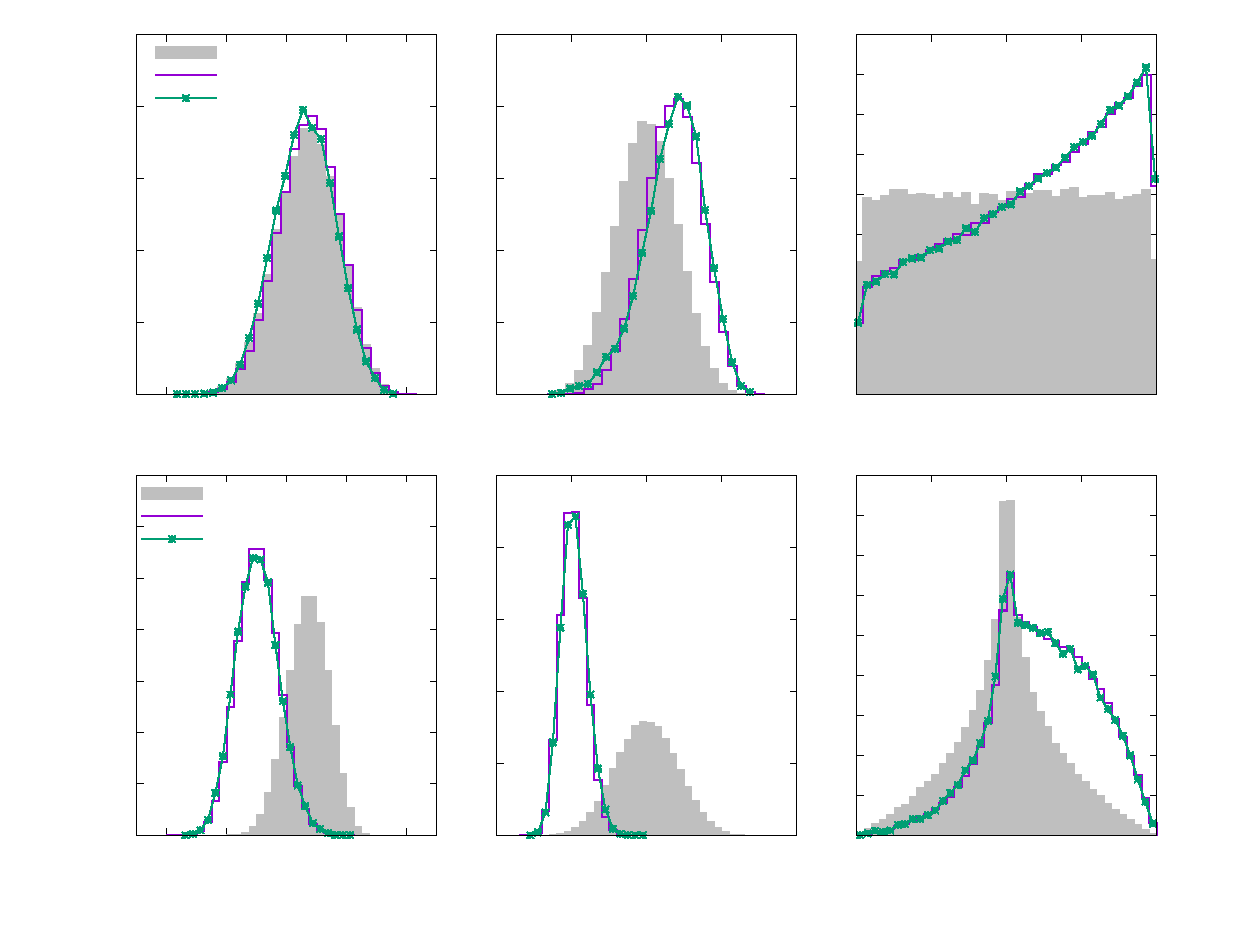
\includegraphics[width={576.00bp},height={432.00bp}]{fig-inc}}%
    \gplfronttext
  \end{picture}%
\endgroup
\end{document}
